\XtoCBlock{Int2Real}
\label{block:Int2Real}
\begin{figure}[H]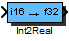
\includegraphics{Int2Real}\end{figure} 

\begin{XtoCtabular}{Inports}
In & Integer input\tabularnewline
\hline
\end{XtoCtabular}


\begin{XtoCtabular}{Outports}
Out & Real output\tabularnewline
\hline
\end{XtoCtabular}

\begin{XtoCtabular}{Mask Parameters}
Scale & Scaling factor from integer to real\tabularnewline
\hline
\end{XtoCtabular}

\subsubsection*{Description:}
Conversion block from integer (fixed point) datatypes to real (floating point) datatypes.

  Out = In * Scale 

% include optional documentation file
\InputIfFileExists{\XcHomePath/Library/General/Doc/Int2Real_Info.tex}{\vspace{1ex}}{}

\subsubsection*{Implementations:}
\begin{tabular}{l l}
\textbf{FiP8\_Float32} & 8 Bit Fixed Point to 32 Bit Floating Point Implementation\tabularnewline
\textbf{FiP16\_Float32} & 16 Bit Fixed Point to 32 Bit Floating Point Implementation\tabularnewline
\textbf{FiP32\_Float32} & 32 Bit Fixed Point to 32 Bit Floating Point Implementation\tabularnewline
\textbf{FiP8\_Float64} & 8 Bit Fixed Point to 64 Bit Floating Point Implementation\tabularnewline
\textbf{FiP16\_Float64} & 16 Bit Fixed Point to 64 Bit Floating Point Implementation\tabularnewline
\textbf{FiP32\_Float64} & 32 Bit Fixed Point to 64 Bit Floating Point Implementation\tabularnewline
\end{tabular}

\XtoCImplementation{FiP8\_Float32}
\index{Block ID!192}
\nopagebreak[0]
% Implementation details
\begin{tabular}{l l}
\textbf{Name} & FiP8\_Float32 \tabularnewline
\textbf{ID} & 192 \tabularnewline
\textbf{Revision} & 0.1 \tabularnewline
\textbf{C filename} & Int2Real\_FiP8\_Float32.c \tabularnewline
\textbf{H filename} & Int2Real\_FiP8\_Float32.h \tabularnewline
\end{tabular}
\vspace{1ex}

8 Bit Fixed Point to 32 Bit Floating Point Implementation

\begin{XtoCtabular}{Controller Parameters}
scale & Scaling factor\tabularnewline
\hline
\end{XtoCtabular}

% Implementation data structure
\XtoCDataStruct{Data Structure:}
\begin{lstlisting}
typedef struct {
     uint16        ID;
     int8          *In;
     float32       Out;
     float32       scale;
} INT2REAL_FIP8_FLOAT32;
\end{lstlisting}

\ifdefined \AddTestReports
\InputIfFileExists{\XcHomePath/Library/General/Doc/Test_Int2Real_FiP8_Float32.tex}{}{}
\fi
\XtoCImplementation{FiP16\_Float32}
\index{Block ID!193}
\nopagebreak[0]
% Implementation details
\begin{tabular}{l l}
\textbf{Name} & FiP16\_Float32 \tabularnewline
\textbf{ID} & 193 \tabularnewline
\textbf{Revision} & 0.1 \tabularnewline
\textbf{C filename} & Int2Real\_FiP16\_Float32.c \tabularnewline
\textbf{H filename} & Int2Real\_FiP16\_Float32.h \tabularnewline
\end{tabular}
\vspace{1ex}

16 Bit Fixed Point to 32 Bit Floating Point Implementation

\begin{XtoCtabular}{Controller Parameters}
scale & Scaling factor\tabularnewline
\hline
\end{XtoCtabular}

% Implementation data structure
\XtoCDataStruct{Data Structure:}
\begin{lstlisting}
typedef struct {
     uint16        ID;
     int16         *In;
     float32       Out;
     float32       scale;
} INT2REAL_FIP16_FLOAT32;
\end{lstlisting}

\ifdefined \AddTestReports
\InputIfFileExists{\XcHomePath/Library/General/Doc/Test_Int2Real_FiP16_Float32.tex}{}{}
\fi
\XtoCImplementation{FiP32\_Float32}
\index{Block ID!194}
\nopagebreak[0]
% Implementation details
\begin{tabular}{l l}
\textbf{Name} & FiP32\_Float32 \tabularnewline
\textbf{ID} & 194 \tabularnewline
\textbf{Revision} & 0.1 \tabularnewline
\textbf{C filename} & Int2Real\_FiP32\_Float32.c \tabularnewline
\textbf{H filename} & Int2Real\_FiP32\_Float32.h \tabularnewline
\end{tabular}
\vspace{1ex}

32 Bit Fixed Point to 32 Bit Floating Point Implementation

\begin{XtoCtabular}{Controller Parameters}
scale & Scaling factor\tabularnewline
\hline
\end{XtoCtabular}

% Implementation data structure
\XtoCDataStruct{Data Structure:}
\begin{lstlisting}
typedef struct {
     uint16        ID;
     int32         *In;
     float32       Out;
     float32       scale;
} INT2REAL_FIP32_FLOAT32;
\end{lstlisting}

\ifdefined \AddTestReports
\InputIfFileExists{\XcHomePath/Library/General/Doc/Test_Int2Real_FiP32_Float32.tex}{}{}
\fi
\XtoCImplementation{FiP8\_Float64}
\index{Block ID!195}
\nopagebreak[0]
% Implementation details
\begin{tabular}{l l}
\textbf{Name} & FiP8\_Float64 \tabularnewline
\textbf{ID} & 195 \tabularnewline
\textbf{Revision} & 0.1 \tabularnewline
\textbf{C filename} & Int2Real\_FiP8\_Float64.c \tabularnewline
\textbf{H filename} & Int2Real\_FiP8\_Float64.h \tabularnewline
\end{tabular}
\vspace{1ex}

8 Bit Fixed Point to 64 Bit Floating Point Implementation

\begin{XtoCtabular}{Controller Parameters}
scale & Scaling factor\tabularnewline
\hline
\end{XtoCtabular}

% Implementation data structure
\XtoCDataStruct{Data Structure:}
\begin{lstlisting}
typedef struct {
     uint16        ID;
     int8          *In;
     float64       Out;
     float64       scale;
} INT2REAL_FIP8_FLOAT64;
\end{lstlisting}

\ifdefined \AddTestReports
\InputIfFileExists{\XcHomePath/Library/General/Doc/Test_Int2Real_FiP8_Float64.tex}{}{}
\fi
\XtoCImplementation{FiP16\_Float64}
\index{Block ID!196}
\nopagebreak[0]
% Implementation details
\begin{tabular}{l l}
\textbf{Name} & FiP16\_Float64 \tabularnewline
\textbf{ID} & 196 \tabularnewline
\textbf{Revision} & 0.1 \tabularnewline
\textbf{C filename} & Int2Real\_FiP16\_Float64.c \tabularnewline
\textbf{H filename} & Int2Real\_FiP16\_Float64.h \tabularnewline
\end{tabular}
\vspace{1ex}

16 Bit Fixed Point to 64 Bit Floating Point Implementation

\begin{XtoCtabular}{Controller Parameters}
scale & Scaling factor\tabularnewline
\hline
\end{XtoCtabular}

% Implementation data structure
\XtoCDataStruct{Data Structure:}
\begin{lstlisting}
typedef struct {
     uint16        ID;
     int16         *In;
     float64       Out;
     float64       scale;
} INT2REAL_FIP16_FLOAT64;
\end{lstlisting}

\ifdefined \AddTestReports
\InputIfFileExists{\XcHomePath/Library/General/Doc/Test_Int2Real_FiP16_Float64.tex}{}{}
\fi
\XtoCImplementation{FiP32\_Float64}
\index{Block ID!197}
\nopagebreak[0]
% Implementation details
\begin{tabular}{l l}
\textbf{Name} & FiP32\_Float64 \tabularnewline
\textbf{ID} & 197 \tabularnewline
\textbf{Revision} & 0.1 \tabularnewline
\textbf{C filename} & Int2Real\_FiP32\_Float64.c \tabularnewline
\textbf{H filename} & Int2Real\_FiP32\_Float64.h \tabularnewline
\end{tabular}
\vspace{1ex}

32 Bit Fixed Point to 64 Bit Floating Point Implementation

\begin{XtoCtabular}{Controller Parameters}
scale & Scaling factor\tabularnewline
\hline
\end{XtoCtabular}

% Implementation data structure
\XtoCDataStruct{Data Structure:}
\begin{lstlisting}
typedef struct {
     uint16        ID;
     int32         *In;
     float64       Out;
     float64       scale;
} INT2REAL_FIP32_FLOAT64;
\end{lstlisting}

\ifdefined \AddTestReports
\InputIfFileExists{\XcHomePath/Library/General/Doc/Test_Int2Real_FiP32_Float64.tex}{}{}
\fi
